\documentclass[a4paper,titlepage,openany,12pt]{report}

\usepackage[T1]{fontenc}
\usepackage[utf8]{inputenc}
\usepackage[francais]{babel}
\usepackage{lmodern}
\usepackage{pxfonts}
\usepackage{graphicx}
\usepackage{lscape}

\title{Projet CPS (MI047) - River City Ransom}
\author{Kevin Coquart \and Quentin Bunel}

\begin{document}

\maketitle

\section*{Introduction}

L'objectif du projet est de réaliser la spécification du jeu River City Ransom,
puis d'implémenter celle-ci (décorateurs, contracts, tests) selon la méthodologie du cours.
Nous avons découpé le travail en 11 services.

Les spécifications ont été redigées dans le format org. C'est un format de l'éditeur Emacs
qui permet de générer facilement des fichiers html ou pdf (voir plus bas).

\section*{Solutions}

\paragraph{}
Un des premiers problèmes qui s'est présenté à nous est qu'il fallait différencier les objets équipables
des objets marchands. En effet, les objets marchands ont un prix et peuvent se vendre, alors que les objets 
équipables doivent contenir un bonus, c'est-à-dire un nombre de points de vie à retirer au personnage cible 
d'un éventuel jet. Notre service Objet déclare uniquement un observateur nom() de type String et possède deux 
sous-services : ObjetEquipable et ObjetMarchand.

Un autre facteur vient cependant modifier la solution : un personnage peut être porté par un autre !
Personnage raffinerait donc ObjetEquipable ? et donc Objet ?
La solution que nous avons choisi a été la création d'un service Chose qui décrit ce qui est portable et 
le bonus apporté. Personnage et ObjetEquipable raffinent tous les deux Chose.
Ainsi, quand on a besoin de manipuler des objets, comme dans les blocs du terrain, on est sûr de ne pas
confondre avec les personnages.

\paragraph{}
Le diagramme ci-dessous représente l'architecture globale de notre projet.
On y voit les liens de raffinement (flèches pointillées) et les liens d'utilisation.
Par exemple, moteurJeu utilise gestionCombat.

\begin{landscape}  % passage en paysage
  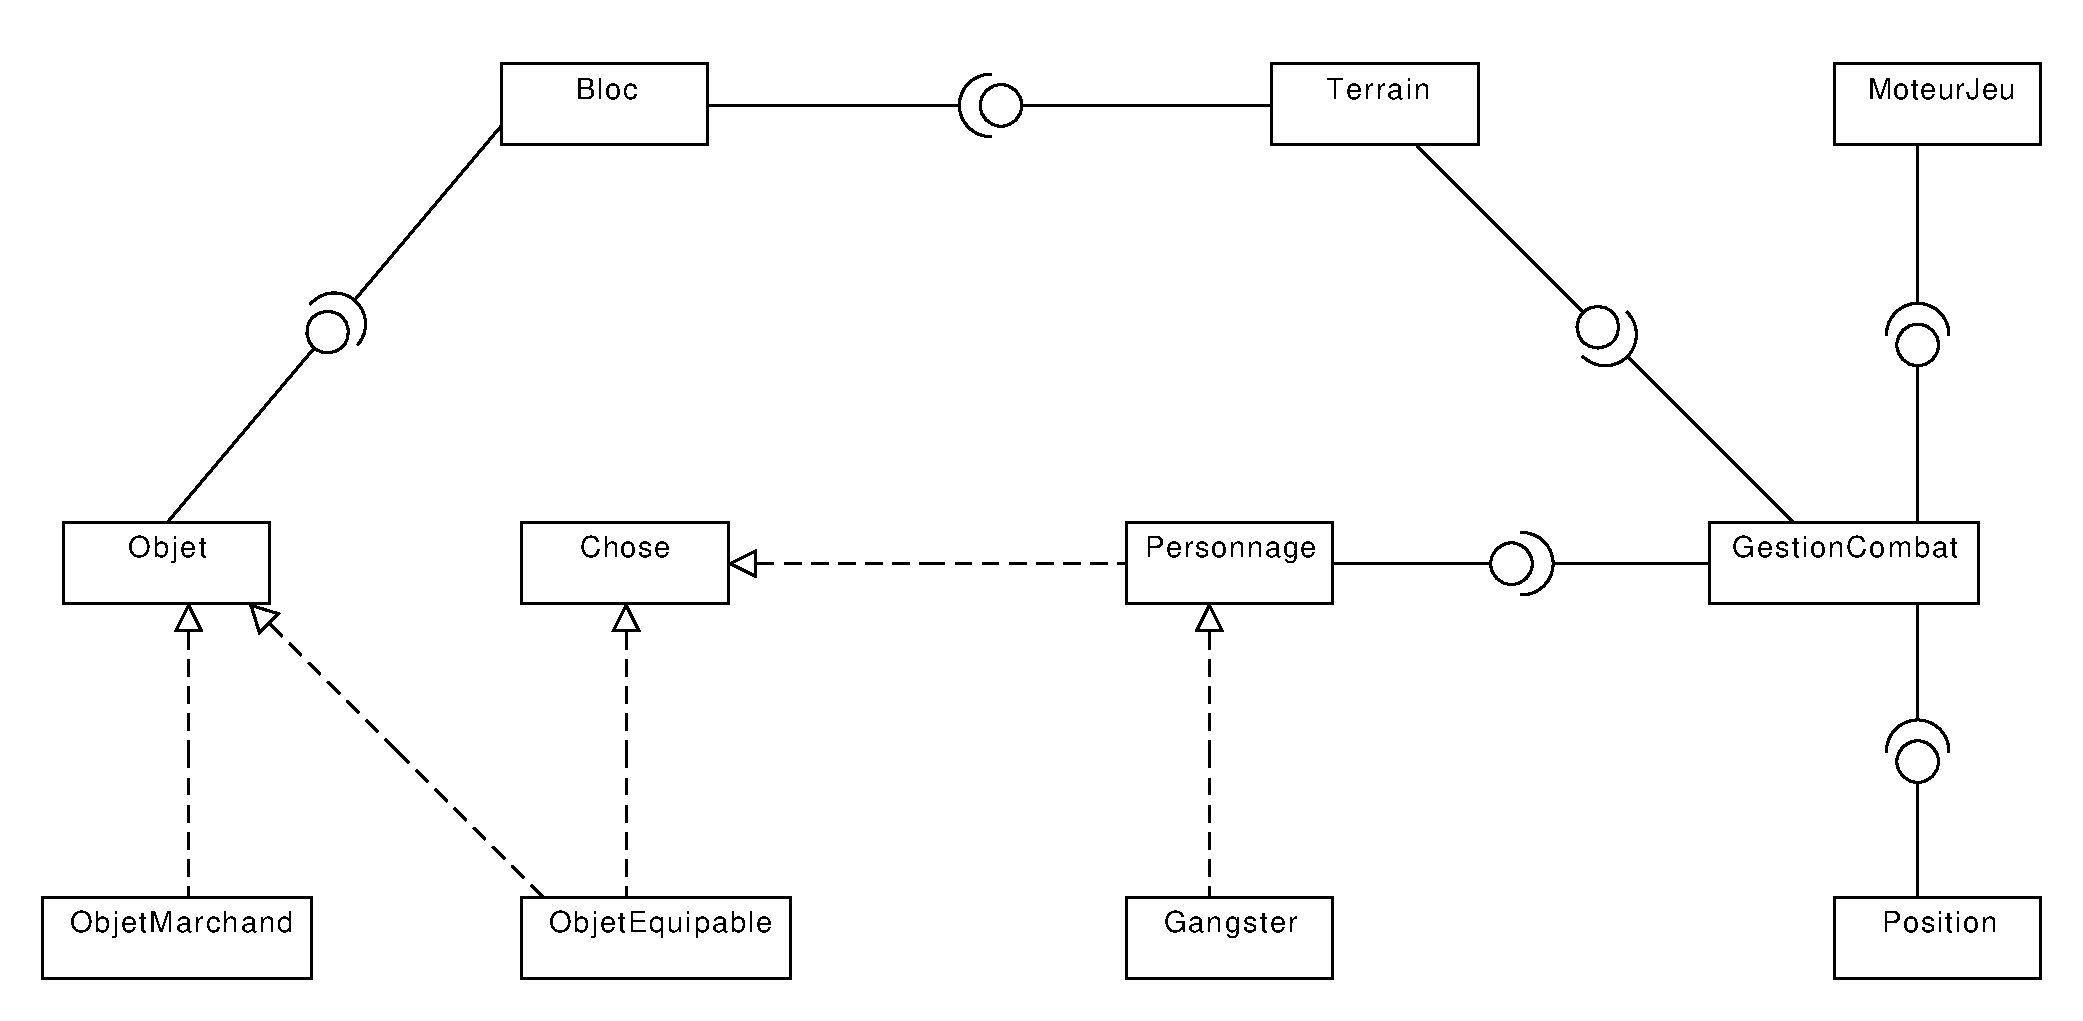
\includegraphics[width=24cm]{../presentation/diagProjetCPS}
\end{landscape}

\paragraph{}
Pour avoir accès aux personnages, dans GestionCombat, nous avons fait le choix d'avoir une Map dont les
clés sont les noms des personnages, et les valeurs les instances de Personnage (ou Gangster). On peut par 
exemple appeler mPerso.get("Alex") pour récupérer Alex.
De plus, la méthode gerer() prend en paramètre une Map<String, COMMANDE> qui associe à chaque personnage
la commande qu'il doit réaliser dans le pas de jeu.

Cela nous a permis d'unifier le traitement des différents types de
pions (Alex, Ryan, Slick et les gangsters).
Grace à leur nom, on a acces a l'objet qui les représente, leur
position, et leur état (gel).
Au total, nous gérons 3 Map pour l'objet, la position et leur état.

\paragraph{}
Nous avons decidé de faire de gestion combat un processus du jeu mais
de ne pas lui donner de pouvoir décision, les décisions viennent du
moteur de Jeu.
Le moteur de jeu donne les commandes pour tout le monde, bot compris.
Il peut aussi ajouter un nouveau nom à la liste des commandes et ainsi
créer un nouveau gangster.
Ce mode de gestion séparé permet de bien différencier le centre de
décision du processus d'avancement. Cela simplifie aussi les
améliorations possibles.
En modifiant moteur jeu l'on peut aisément faire une nouvelle
implémentation ou les gangsters deviendraient controlables. Et pourquoi
pas en faire une version réseau avec 2 camps, les gentils et les méchants.


\section*{Annexes}

Vous trouverez ci-joint :
\begin{itemize}
\item Dans /spec, les specifications au format org et le Makefile pour générer les formats html et pdf (voir README.txt)
\item Dans /tests, les tests au format org et le Makefile pour générer les formats html et pdf (voir README.txt)
\item Le code des services, décorateurs, contracts, tests et implémentation dans /src
\item Des archives jar exécutables dans /jars
\end{itemize}
Note : les makefile ont été préalablement exécutés.

\section*{Version Bogue}
\paragraph{}
Il y a deux implémentations boguées, celle de personnage dont les
contrats renvoient de jolies erreurs.
Et celle de gestion combat, pour celle-ci, le contrat ne pouvant
verifier les passages en erreur, ne produit pas d'exception par contre
les tests renvoient de jolis messages indiquant qu'il y a un soucis.



\section*{Conclusion}

\paragraph{}
Le jeu est fonctionnel, il n'est surement pas exempt de bogue. Nous
avons essayé plusieurs scenarios sans aucun probleme. L'interface
graphique est assez minimaliste, quelques améliorations possibles :
\begin{itemize}
\item l'ajout du pas de jeu dans une barre d'état
\item une boîte d'alerte avec le résultat final
\item la gestion de l'affichage des points de vie
\end{itemize}
Bien sûr les graphismes ne sont pas fous, des petits carrés de couleurs
diverses et variées mais l'ensemble reste cohérant et compréhensible.
Le jeu est entièrement jouable au clavier.


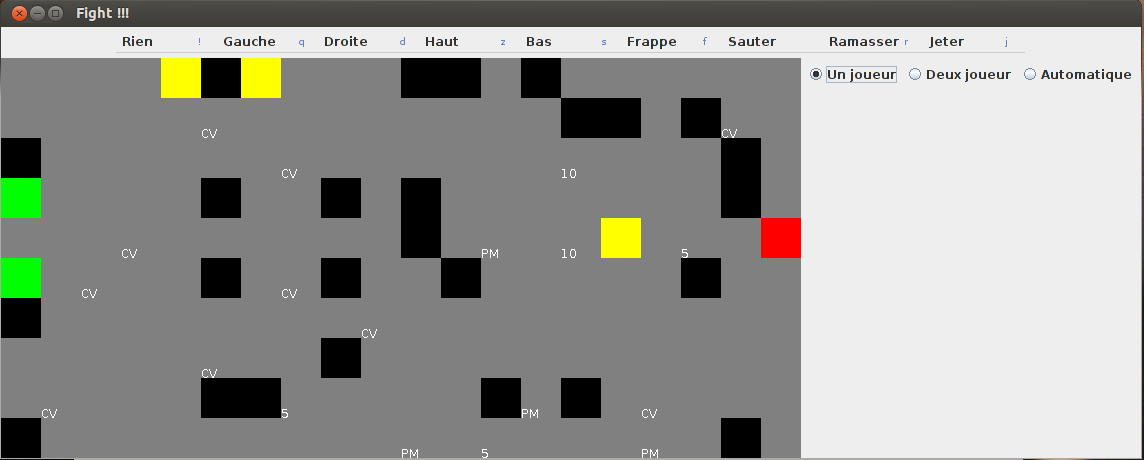
\includegraphics[scale=0.3]{../saved2}


La figure ci-dessus est une capture d'écran du jeu.
Le personnage que nous contrôlons est Alex (carré vert du haut).


\section*{Notice}
\paragraph{}
Le jeu se partage en 3 modes de jeu :
\begin{itemize}
\item automatique
\item un joueur
\item deux joueurs
\end{itemize}

\paragraph{}
Pour changer le comportement des personnages non contrôlés il faut
aller voir la classe tools.GenerateurCmd .
Il existe deux codes pour la meme méthode, une version intelligent qui
va plus souvent à se deplacer puis frapper de temps à autre, ainsi
qu'une version beaucoup plus simple. Dans cette dernière, on peut
basculer en commentant/décommantant dans un mode ou tout le monde est
beau, tout le monde est gentil, la commande renvoyée est RIEN. Ou bien
c'est un random sur un tableau de commandes donné, à nous de choisir
les commandes du tableau.

\paragraph{}
Pour jouer, il suffit de choisir son mode de jeu, le mode 1 joueur est
selectionné au depart. Puis choisir la commande à effectuer (clavier
ou souris).
En mode deux joueurs, il faut choisir deux commandes, l'une à la suite
de l'autre.


\section*{Connaissances acquises}
\paragraph{}
Ce projet nous a permis de decouvrir un aspect qui nous était méconnu
jusqu'à présent, le monde des spécifications.
Au fil de notre scolarité, nous découvrons l'aspect projet petit à
petit.
Au debut sur des projets simples, nous implémentions la solution sans
analyse préalable puis par la suite avec l'ecriture des algorithmes
compliqués pour savoir sur quelle base partir.
Ensuite, nous avons ajouté l'UML à nos compétances, un travail plutôt
long et fastidieux pour le gain qu'il apporte. Les outils à notre
disposition à la fac ne nous permettant pas de gagner réelement du
temps en passant par ces structures.
Enfin grâce à cette UE nous avons découvert les spécifications.

\paragraph{}
Créer des spécifications pour chaque service puis des tests sur
chacun est aussi un travail assez fastidieux mais bien plus complexe
et complet. Par la suite la plupart de l'implémentation est triviale.
Les tests permettent par la suite de vérifier son travail et contaster
les erreurs pour les corriger.
Une fois ces erreurs resolues, la mise en commum des services et l'essai
du jeu se sont passés sans soucis.

\paragraph{}
Nous retenons plusieurs choses de ce projet, premièrement, il est
difficile de faire un jeu en 3 semaines.
Deuxièment, nous ne sommes pas graphistes et cela se remarque très
vite.
Pour finir nous avons découvert le monde des spécifications avec une
approche proche de l'industrie, l'on produit une spécification
complète. Puis quelqu'un se charge de l'implémentation et pour finir
avec nos tests on valide notre travail.
Bien sûr dans le cadre de ce projet, l'implémentation est faite par
nous-même, cela d'ailleurs simplifie grandement la compréhension des
spécifications.


\end{document}
